\documentclass[conference]{IEEEtran}
\IEEEoverridecommandlockouts
% The preceding line is only needed to identify funding in the first footnote. If that is unneeded, please comment it out.
\usepackage[utf8]{inputenc}

\usepackage{cite}
\usepackage{amsmath,amssymb,amsfonts}
\usepackage{algorithmic}
\usepackage{graphicx}
\usepackage{textcomp}
\usepackage{xcolor}
\usepackage{xspace}
\usepackage{paralist}
\usepackage{float}
\usepackage{booktabs}
\usepackage{hyperref}

\def\BibTeX{{\rm B\kern-.05em{\sc i\kern-.025em b}\kern-.08em
    T\kern-.1667em\lower.7ex\hbox{E}\kern-.125emX}}
\begin{document}

\newcommand{\tool}{\textsc{SALVO}\xspace}
\newcommand{\challenge}{2021 IEEE Autonomous Driving AI Test Challenge\xspace}
\newboolean{showcomments}
\setboolean{showcomments}{true}         
%\setboolean{showcomments}{false} 
\ifthenelse{\boolean{showcomments}}
  {\newcommand{\nb}[2]{
  \fbox{\bfseries\sffamily\scriptsize#1}
     {\sf\small$\blacktriangleright$\textit{\textcolor{red}{#2}}$\blacktriangleleft$}
   }
  }
  {\newcommand{\nb}[2]{}
   \newcommand{\cvsversion}{}
  }

\newcommand\alessio[1]{\nb{Alessio}{#1}} 
\newcommand\vuong[1]{\nb{Vuong}{#1}} 
\newcommand\stefan[1]{\nb{Stefan}{#1}} 

%\title{\tool: Automated Generation of Diversified Tests for Self-driving Cars based on Photo-Realistic Maps}
\title{\tool: Automated Generation of Diversified Tests for Self-driving Cars from Existing Maps}



\author{
\IEEEauthorblockN{Vuong Nguyen}
\IEEEauthorblockA{\textit{University of Passau} \\
Passau, Germany \\
nguyen58@ads.uni-passau.de}
\and
\IEEEauthorblockN{Stefan Huber}
\IEEEauthorblockA{\textit{University of Passau} \\
Passau, Germany \\
stefan.huber.niedling@outlook.com}
\and
\IEEEauthorblockN{Alessio Gambi}
\IEEEauthorblockA{\textit{University of Passau} \\
Passau, Germany \\
alessio.gambi@uni-passau.de}
}

\maketitle

\begin{abstract}
% Testing self-driving car software using photo-realistic and accurate physical simulators is becoming a widely adopted practice. Simulators enable the automated execution of many tests that possibly implement safety-critical driving scenarios that are too dangerous to put into practice. However, despite the speed-up achieved by using simulators, fundamental challenges are yet to be addressed before achieving cost-effective testing of self-driving cars.
% %
% In this paper, we present \tool, an approach to automated self-driving car software testing that addresses some of those challenges. Specifically, \tool
% \begin{inparaenum}[(i)]
% \item systematically identifies relevant driving scenarios among a myriad of potential driving scenarios that can be defined over existing maps;
% \item selects driving scenarios that reduce testing efforts while ensuring quantifiable different behaviors, and 
% \item automatically generates test cases that implement those diversified driving scenarios.
% \end{inparaenum}
% %
% We demonstrated \tool in the \challenge
% by testing state-of-the-art self-driving car software using an industrial driving simulator.
% In a matter of minutes, \tool analyzed five maps of different complexity levels (from $2$ to more than $15$ intersections), identified more than $1100$ relevant driving scenarios, and selected on average half of them for the execution.
% %
% The evaluation results showed that tests cases generated by \tool from the selected driving scenarios resulted in quantifiable different trajectories followed by the test subject and exposed issues in it.

%For testing self-driving cars simulations are heavily utilized since these allow running many simulations at once and allow enforcing critical situations without endangering any other drivers or pedestrians.
%For increasing the quality of tests photo-realistic maps and accurate physical simulators are a widely adopted and still growing practice.
%However, despite these advantages there are still fundamental challenges including cost-effectiveness and further increasing the degree of automation for finding or generating critical tests.\\
%This paper presents \tool, an approach
%(1) to systematically identify relevant driving scenarios among the myriad of potential driving scenarios,
%(2) to select scenarios that reduce the required overall testing efforts by ensuring quantifiability and diversity of the expected behaviours of self-driving cars for succeeding scenarios and
%(3) to generate those test cases.\\
%We demonstrated \tool at the \challenge by running state-of-the-art self-driving car software in an industrial driving simulator against our generated test cases.
%In a matter of minutes, \tool analyzed five maps of different complexity (from 2 to more than 15 intersections), identified more than 1100 relevant driving scenarios and selected on average half of them for actual test executions.
%The evaluation results showed that the generated test cases resulted in quantifiable and diverse trajectories and exposed issues of the self-driving car software.

Simulation-based tests are more cost-effective and less dangerous than field tests; hence, they are becoming the norm for thoroughly testing self-driving cars in virtual environments. High-quality simulation-based testing requires physically accurate computer simulations,  detailed and photo-realistic maps, and systematic approaches for generating tests. Moreover, since creating detailed maps is a manual process, they are expensive, and testers should avoid wasting such valuable resources, for example, by generating irrelevant test cases. To address those issues, we propose \tool a fully automated approach to identify quantifiably diverse and critical driving scenarios that can be instantiated on existing high-definition maps and implement them in an industrial driving simulator as executable test cases.
The evaluation of \tool in the context of the \challenge showed that it could analyze maps of different complexity and identify many critical driving scenarios in minutes. Furthermore, the tests \tool generated stressed a state-of-art self-driving car software in quantifiably diverse ways and exposed issues with its implementation.
\end{abstract}

 \begin{IEEEkeywords}
Test Case Generation, Autonomous Vehicles, Software-in-the-loop, Diversity, Feature Space
 \end{IEEEkeywords}

\section{Introduction and Motivation}
Self-driving cars promise to reduce traffic accidents \cite{peden2016status}, increase fuel efficiency~\cite{zamzuri2016current} and enhance comfort~\cite{harper2016estimating}.
Testing self-driving car software is laborious and challenging since self-driving car's development is still in an early stage, and there is a lack of standardized procedures and established approaches \cite{gambi2019generating}. Therefore, many researchers and organizations are currently investigating testing approaches to increase the quality of autonomous vehicles before they roam the thoroughfares.
%
Naturalistic field operational testing is a popular approach to validate and verify the safety of autonomous vehicles that leaves them free to drive on actual roads. However, as discussed by Kalra and Paddock~\cite{kalra2016driving}, this method is inefficient since relevant execution conditions (e.g., traffic situations that lead to traffic accidents) are hard to observe and ineffective as dangerous situations are impossible to recreate. Those, in turn, make limit the replicability of natural field operational tests' results ~\cite{hasenau2019virtual}. An alternative approach is virtual testing, also known as simulation-based testing, which uses computer simulations to generate diverse test cases to challenge the self-driving software involving traffic patterns and numerous virtual road conditions~\cite{hasenau2019virtual}. Virtual testing enables automated test execution and can expose problems in autonomous software, including perception, planning, and decision-making systems. However, it requires the availability of accurate geometrical models (e.g., 3D models with textures and material properties) to achieve photo-realism, i.e., to close the simulation-to-reality gap~\cite{9207173}, and detailed road maps. Consequently, cartography is an essential building block to conduct thorough virtual testing of autonomous vehicles~\cite{althoff2018automatic}.  Artists and domain experts cooperate to create those models and maps following a manual, laborious, and expensive process.

\begin{figure}[t]
  \centering
    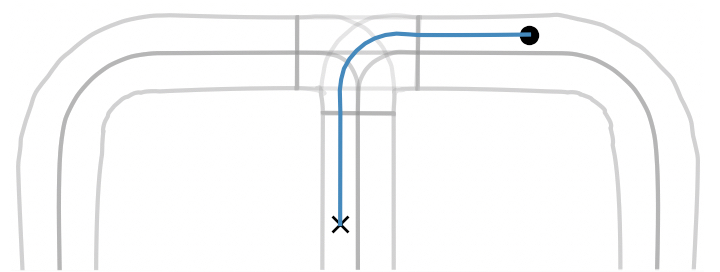
\includegraphics[width=0.3\textwidth]{images/cubetown_1}
    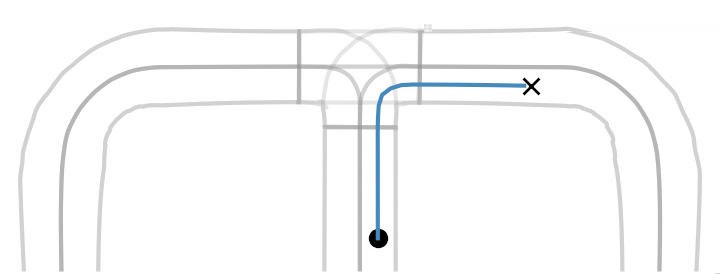
\includegraphics[width=0.3\textwidth]{images/cubetown_2}
    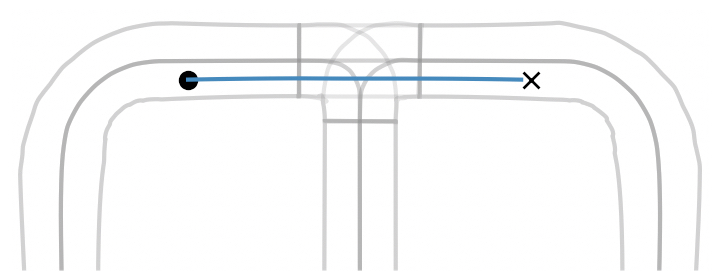
\includegraphics[width=0.3\textwidth]{images/cubetown_3}
  \caption{Sample driving scenarios generated by \tool from an intersection in the Cube Town map available for the \challenge. Driving scenarios begin before entering an intersection~($\bullet$) and end after passing it~($\times$). Top: left turn; Middle: right turn; Bottom: straight through.}
  \label{fig:samples-cubetown}
\end{figure}

Detailed road maps consist of roads composed of lanes, their interconnections (e.g., intersections, junctions), and traffic regulations controlling them (e.g., speed limit, traffic direction); hence, they allow testers to create rich, coherent, and diversified driving scenarios~\cite{althoff2018automatic,bender2014lanelets}. 
%
Among the existing formats to model road maps, in this work, we rely on the notion of \emph{lanelets}~\cite{bender2014lanelets}, an innovative concept for road representation adopted by many (see Section~\ref{subsect:lanelets}).
%
Specifically, we rely on the semantics encoded in the lanelets representation of existing maps to identify intersections and create relevant driving scenarios around and across them. In other words, we abstract existing maps into the lanelets format to generate relevant and diversified \emph{abstract} driving scenarios. Next, we instantiate those abstract scenarios into concrete ones and generate simulation-based test cases that automatically challenge the autonomous vehicle's software in existing driving simulators.

In this paper, we present \tool that implements our approach and summarize its evaluation in the context of the \challenge.
\tool, which is dubbed after the author's first names ---Stephan, Alessio, and Vuong--- and means ``safe'' in Italian, works under the consideration that because manually generated road maps are costly and valuable, testers must use (and re-use) them wisely and extensively. 
Consequently, and in contrast to many existing test case generators (e.g., ~\cite{DBLP:conf/icse/GambiMF19,DBLP:conf/icse/HuynhGF19,DBLP:conf/sigsoft/RiccioT20,DBLP:conf/issta/ZohdinasabRGT21,DBLP:conf/sbst/PanichellaGZR21}) that procedurally generate virtual roads, it leverages existing maps to generate as many tests as possible.
%
However, since generating virtual tests without any guidance is not cost-effective either because not all the generated tests are relevant or because many tests are similar to each other, \tool follows a systematic approach to generate only relevant test cases and maximize their diversity.

The current implementation of \tool takes existing maps in OpenDrive format~\cite{dupuis2010opendrive}, generates abstract driving scenarios involving intersections, and selects among them those that result in quantifiably different ego-vehicle trajectories (see Figure~\ref{fig:samples-cubetown}). Finally, it instantiates the selected scenarios in the industrial driving simulation SVL~Simulator~\cite{rong2020lgsvl} as test cases and automatically executes them.
%
We released \tool freely at the following link:
\begin{center}
\href{https://github.com/TrackerSB/IEEEAITestChallenge2021}{https://github.com/TrackerSB/IEEEAITestChallenge2021}
\end{center}


\section{LGSVL Simulator}
\label{subsect:lgsvl}
The LGSVL is a high fidelity simulator that providing full-stack simulation to challenge the autonomous driving software \cite{rong2020lgsvl}. The core simulation engine is based on the Unity game engine \cite{rong2020lgsvl}, one of the best solutions for high fidelity, developer-friendly, cost-effective simulation environments in the industry \cite{craighead2008using}. The simulator provides a reliable communication bridge that allows the exchange of ROS, ROS2, and Cyber RT messages between the simulator and other Autonomous Driving stacks \cite{rong2020lgsvl}. Thus, it can enable software engineers to quickly testing their self-driving software without driving actual vehicles in such common stacks as Autoware and Baidu Apollo \cite{rong2020lgsvl} as illustrated in the Figure~\ref{fig:apollosim}. Moreover, additional features such as easily customize sensors, build and manage new controllable objects, adjust the core simulator' modules, and generate diversified scenarios of particular environments, the simulator can empower various simulation applications for autonomous driving and more \cite{rong2020lgsvl}.

\begin{figure}[tp]
  \centering
    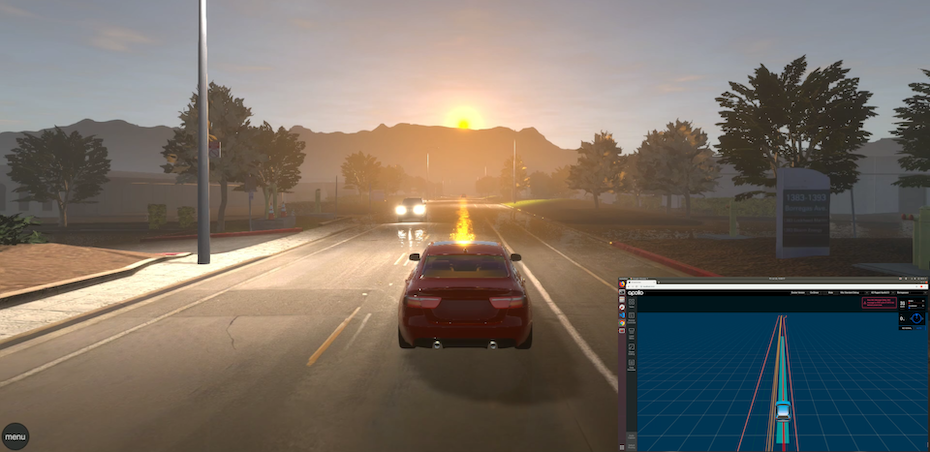
\includegraphics[width=0.5\textwidth]{images/apollo-sim}
  \caption{
    Apollo running with LGSVL Simulator, via LGSVL Simulator Website (\href{https://www.svlsimulator.com/docs/archive/2020.06/apollo-master-instructions}{https://www.svlsimulator.com/docs/archive/2020.06/apollo-master-instructions}).
    }
  \label{fig:apollosim}
\end{figure}


\section{Lanelets}
\label{subsect:lanelets}
Lanelets are a novel concept to represent the map in both topological and geometrical terms that roughly correspond to (segments of) road lanes~\cite{bender2014lanelets}. Lanelets comprise a set of atomic, interconnected, and \emph{drivable} road segments defined by a left and right bound. Bounds are implemented as polylines (i.e., list of points) and implicitly define the traffic direction, which helps determine the route from the given point to the predefined destination~\cite{PekIV20}.

\begin{figure}[H]
  \centering
    \includegraphics[width=0.5\textwidth]{images/lanelets_01}
  \caption{An example of lanelets \cite{althoff2018automatic}.}
  \label{fig:lanelets}
\end{figure}

As illustrated in Figure~\ref{fig:lanelets}, connecting lanelets establishes semantic relations among them and gives rise to road segments and complex road networks that include merge/join and intersections. For example, \emph{adjacent} lanelets share a bound while \emph{preceding/following} lanelets share start point and endpoint in accordance to their traffic directions~\cite{althoff2018automatic}. Notably, lanelets can overlap and share the same start point and endpoint; consequently, they can form complex intersections~\cite{Althoff2017a} and can be used as an intermediate format to represent existing maps~\cite{althoff2018automatic}.
%
As we detail later, \tool relies on those features to translate existing maps into the lanelets format, identify intersections, and define (abstract) driving scenarios.

\section{Automatically Generating Diversified Tests from Existing Maps}
This section describes our approach and the generated test scenarios. The following sections, instead, summarize achieved results and found problems.

\begin{figure*}[t]
\minipage{0.32\textwidth}
\includegraphics[width=\linewidth]{images/distance_cubetown_2}
\endminipage\hfill
\minipage{0.32\textwidth}
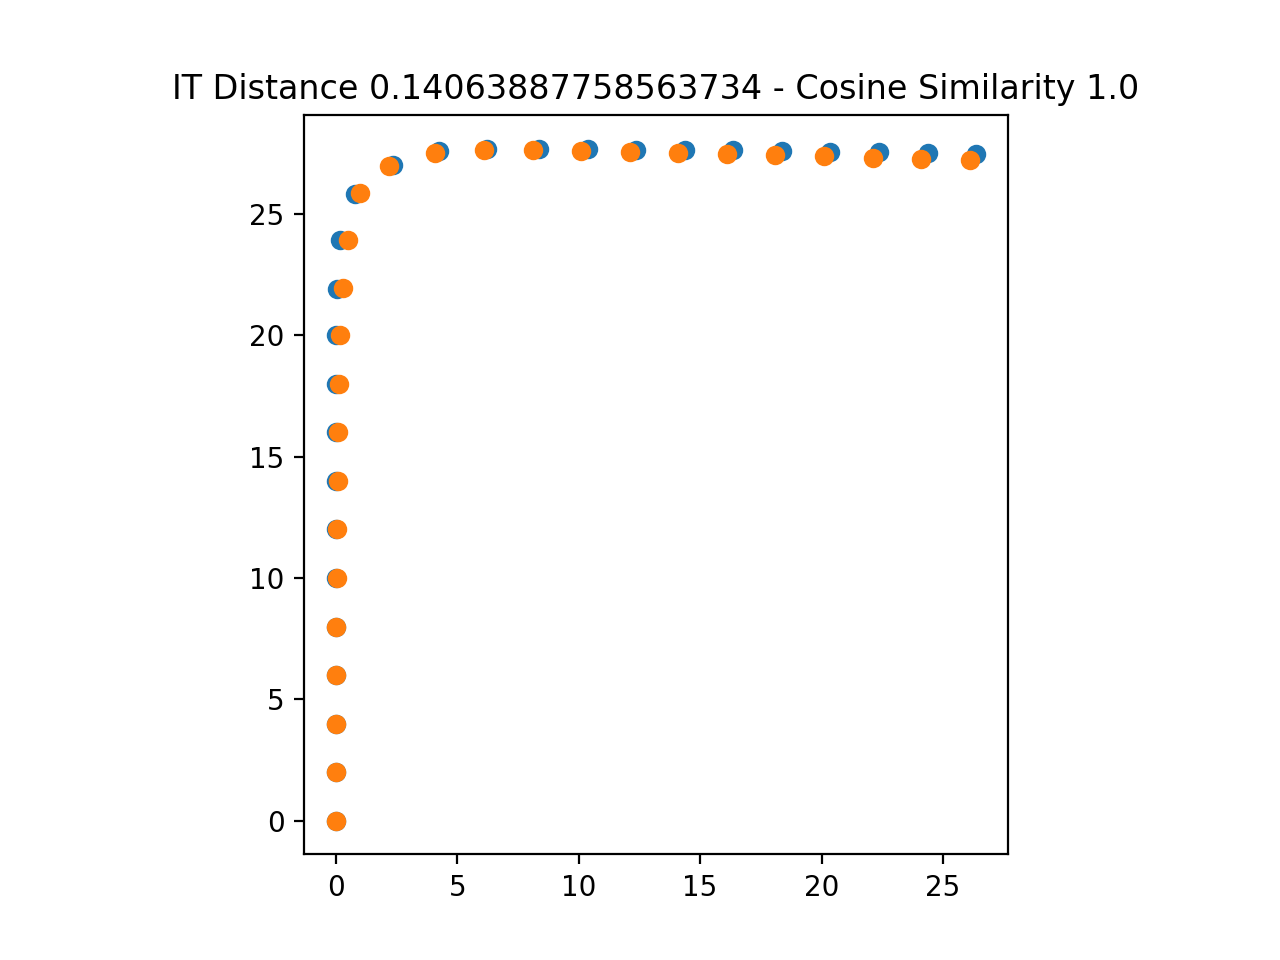
\includegraphics[width=\linewidth]{images/distance_cubetown_1}
\endminipage\hfill
\minipage{0.32\textwidth}%
  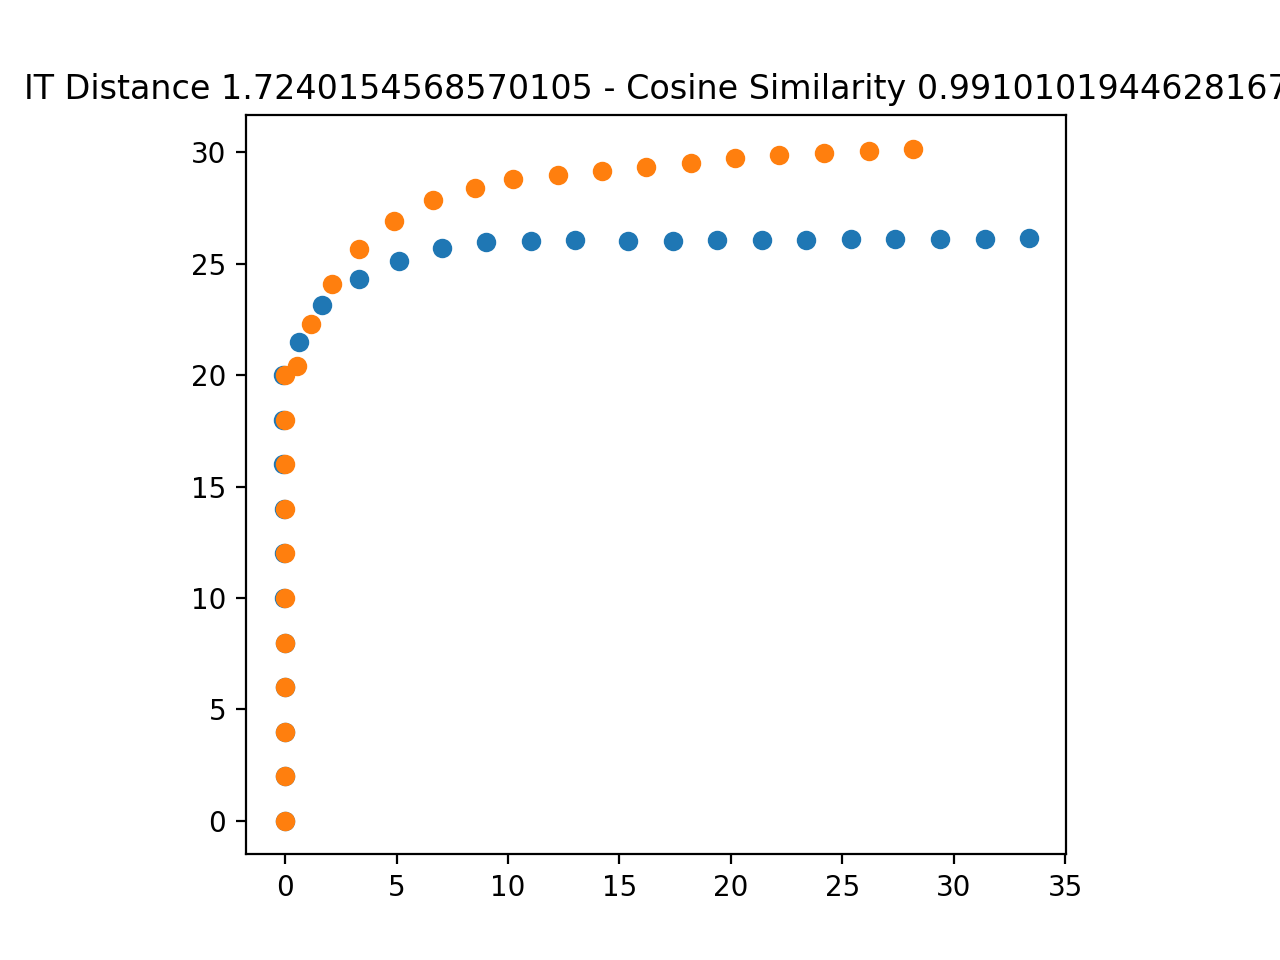
\includegraphics[width=\linewidth]{images/distance_ba_2}
\endminipage
\caption{Examples of trajectories at increasing levels of similarity. We generated the leftmost (dist=$0$) and central (dist=$0.14$) examples from the Cube Town map, while we generated the rightmost example (dist=$1.72$) from the Borregas Avenue map.}
\label{fig:similarity}
\end{figure*}


\subsection{\tool in a Nutshell}
\tool is entirely automatic and can generate test cases that stress the ego-vehicle in many different ways, possibly involving obstacles that partially or completely occlude the lane in which the ego-vehicle is driving. 

Given a map in OpenDrive\footnote{\href{https://www.asam.net/standards/detail/opendrive/}{https://www.asam.net/standards/detail/opendrive}}  format, \tool 
\begin{inparaenum}[(1)]
\item identifies the intersections in the map and 
\item generates abstract driving scenarios that force the ego-vehicle to plan legal trajectories to cross those intersections. Next, \item it selects driving scenarios that correspond to quantifiably different trajectories and
\item generates test cases implementing them. 
Finally, \item it generates even more test cases by placing static obstacles, i.e., parked Non-Playable Characters (NPC) vehicles, in front of the ego-vehicle.
\end{inparaenum}

The following sections detail each step of the proposed approach.

\subsection{Identifying Intersections}
We use the opendrive2lanelet library~\cite{althoff2018automatic} to translate the original maps from the OpenDrive to the lanelets format. As discussed in Section~\ref{subsect:lanelets}, the lanelets organizes its format by relations using follow and adjacent and provides geometrical information (e.g., the shape of each lanelet) and semantic information. 

Despite this, its structure does not explicitly capture intersections; hence \tool implements a heuristic to identify them: First, it uses the geometric information about lanelets to identify overlapping lanelets, which are named as a predecessor, an intersection and a successor. Since overlapping lanelets are likely to belong to the same intersection, \tool groups lanelets that (transitively) overlap together, as demonstrated in Figure~\ref{fig:intersection_a}
%
\begin{figure}[H]
  \centering
    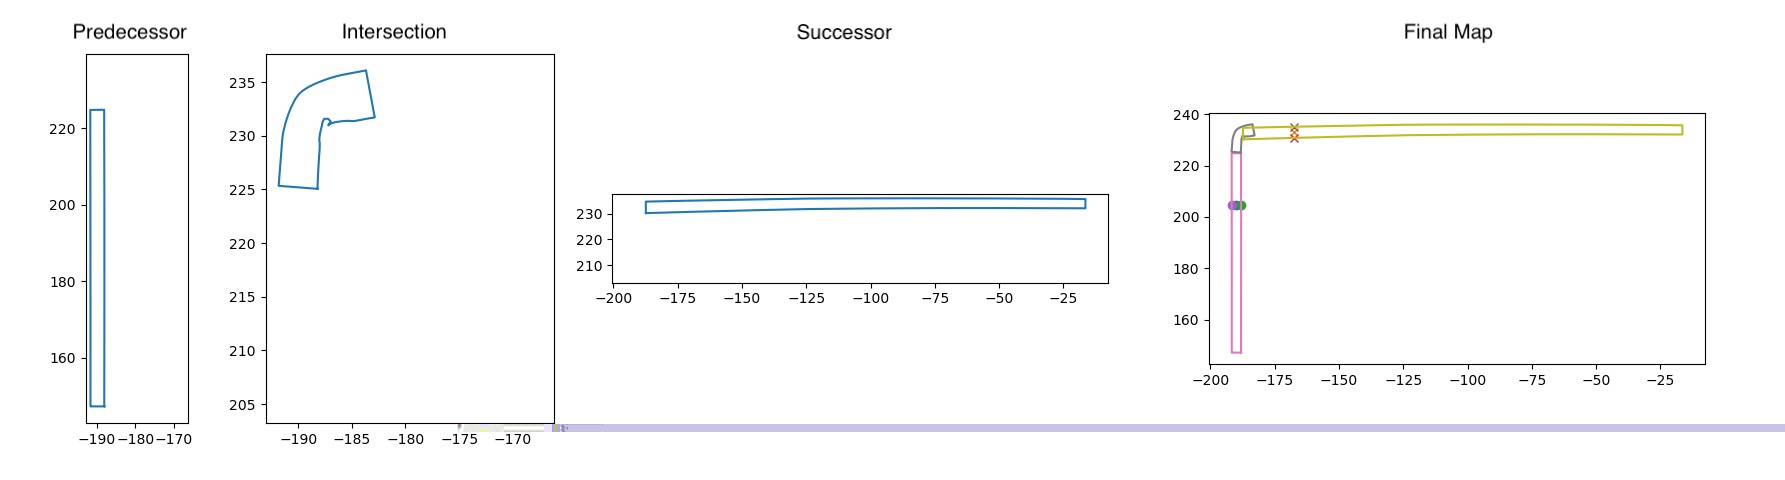
\includegraphics[width=0.5\textwidth]{images/intersection01}
  \caption{An example of an intersection constructed by Salvo.}
  \label{fig:intersection_a}
\end{figure}

The intersections identified this way may be incomplete because some of the lanelets that logically belong to large and complex intersections may not overlap with the other lanelets already assigned to those intersections. Therefore, \tool identifies the missing lanelets as those that are adjacent to the lanelets already assigned to an intersection and include them. As a result, having identified the lanelets that compose intersections, \tool proceeded by generating driving scenarios can force the ego-vehicle to cross them.

\subsection{Generating Relevant Scenarios}
Legal trajectories across intersections such as the ones reported in Figure~\ref{fig:samples-cubetown} define relevant driving scenarios. Legal trajectories follow the traffic directions encoded into the lanelets. Additionally, we limit \tool to consider the simplest form of legal trajectory, i.e., those that do not require the ego-vehicle to change lanes to pass the intersections. Therefore, one typical generated driving scenario will start on a given lane \emph{before} entering an intersection, continue on the same lane across the intersection, and end on the (logically) same lane \emph{after} the intersection.
%
\begin{figure}[H]
  \centering
    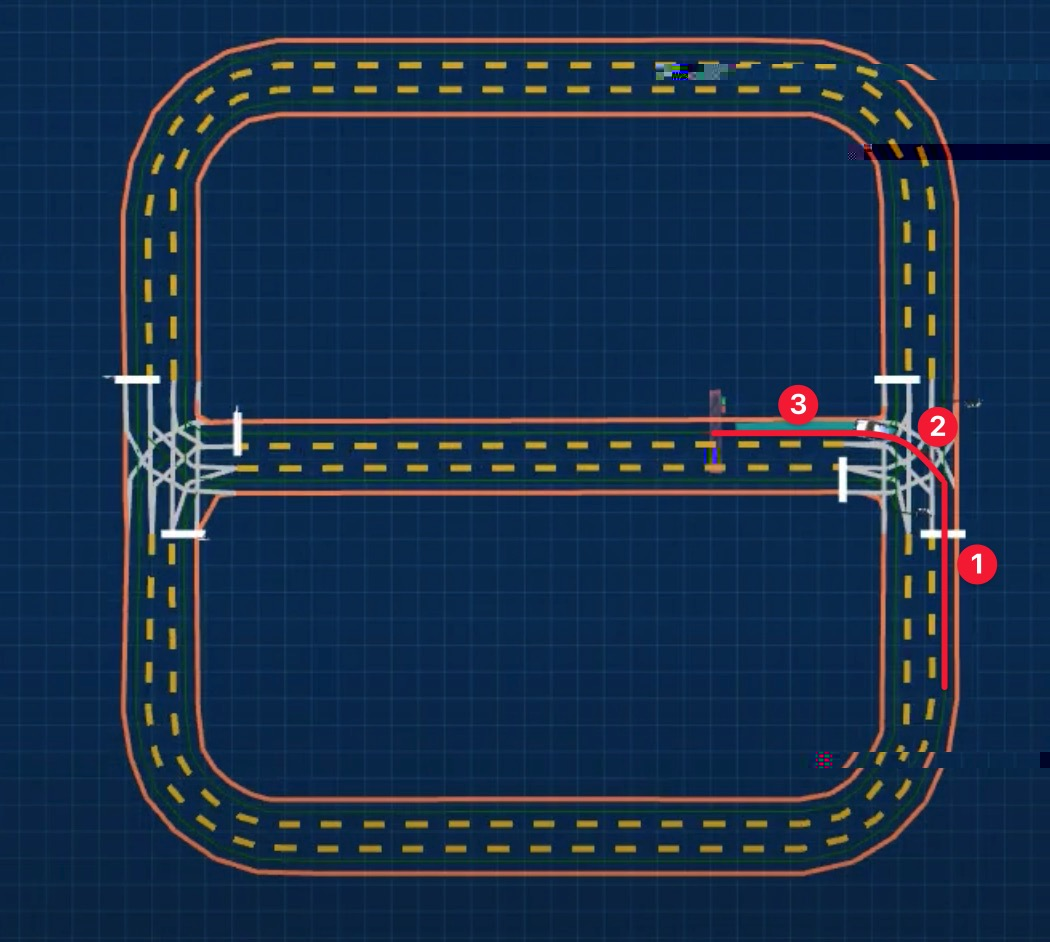
\includegraphics[width=0.5\textwidth]{images/lanelet01}
  \caption{An example of parts of intersection constructed by Salvo. (1) Starting on a given lane, (2) Entering an intersection, (3) Continue on the same lane.}
  \label{fig:intersection_sf}
\end{figure}

\tool generates driving scenarios by selecting the lanelets that belong to an intersection (Figure~\ref{fig:intersection_sf}) and then including those lanelets outside the intersection that \emph{precede} and \emph{follow} the selected ones. Notably, because intersections have various configurations (e.g., number of entering and exiting lanes), the generated driving scenarios indeed force the ego-vehicle to turn left, turn right, or go straight through the intersection.

The generated scenarios are composed of the smallest number (i.e., three) of lanelets. This feature arguably increases the understandability of the resulting test cases but does not necessarily guarantee fast test executions. The lanelets that precede and follow an intersection might be extensive; hence, it may require some time to be fully traversed. Therefore, to reduce execution time, \tool places the ego-vehicle at a fixed distance before entering the intersection and sets the target position to reach at a fixed distance after passing the intersection. Because those distances are configurable, testers can control the duration of test executions and make them more predictable.


\subsection{Selecting Diversified Scenarios}
Up to this point, \tool has not considered the diversity of scenarios. It simply generates as many scenarios as possible to explore the possibilities offered by the input road map. However, many trajectories may stress the ego-vehicle similarly, for example, by forcing it to drive straight through the same intersections from multiple directions. Therefore, \tool filters out test cases that are too similar to each other; hence, improving testing cost-efficiency.

This paper studies two (greedy) approaches for filtering out similar test cases based on distance and feature maps.

\subsubsection{Filtering Similar Scenarios by Similarity}
The first approach to select diversified scenarios is based on computing the similarity of the ego-vehicle' trajectories imposed by the driving scenarios. The chosen metric is Levenshtein distance because it can provide a numerical representation of how different two trajectories are by measuring how many \emph{edits} are required to change one trajectory into the other. Since each trajectory is an array of points, so an \emph{edit} could be an insertion, a deletion, or a substitution of a point. In theory, Levenshtein distance is calculated by initializing an  $m\times n$ matrix where each cell contains the Levenshtein distance between the first $m^{th}$ points of one trajectory and the first $n^{th}$ points of other. The goal is to compute and fill out the entire matrix from the upper left to the lower right corner. Following this way, the number in the bottom-right corner will be Levenshtein distance between both trajectories.
%

Specifically, \tool calculates the iterative Levenshtein distance between pairs of trajectories and discards driving scenarios whose trajectories are not distant enough from (i.e., they are too similar to) the trajectories of the driving scenarios already selected (see Figure~\ref{fig:similarity}).
%
Testers can control the similarity between the trajectories using a configurable threshold to create larger or smaller test suites. 


A similar approach to select diverse trajectories was followed by Zohdinasab and co-author in a pilot study to identify road features relevant for testing lane keeping systems~\cite{DBLP:conf/issta/ZohdinasabRGT21}.
As \tool, they took inspiration for the computation of the iterative Levenshtein distance from the work of Riccio and Tonella~\cite{DBLP:conf/sigsoft/RiccioT20}.

\subsubsection{Filtering Driving Scenarios using Feature Maps}
The second approach to select diversified scenarios is based on the feature maps defined by Zohdinasab et al.~\cite{DBLP:conf/issta/ZohdinasabRGT21}. 
%
\tool generates numerous driving scenarios containing different types of trajectories and features such as minimum curvature and direction coverage capturing high-level characteristics of those trajectories, which can be used to build feature maps. Those maps place driving scenarios in a two-dimensional space according to the values taken by their features.
%
Intuitively, trajectories with similar features are placed in nearby cells, whereas trajectories with different features are placed in distance cells (see Figure~\ref{fig:feature-maps}).

\begin{figure*}[t]
\minipage{0.32\textwidth}
\includegraphics[width=\linewidth]{images/feature_cubetown}
\endminipage\hfill
\minipage{0.32\textwidth}
\includegraphics[width=\linewidth]{images/two_roads_same_cell.png}
\endminipage\hfill
\minipage{0.32\textwidth}%
  \includegraphics[width=\linewidth]{images/roads_different_cell.png}
\endminipage
\caption{Left: Example of feature map distance coverage (dc) $\times$ min radius (mr) generated by \tool from the Cube Town map. Central: Trajectories sampled from the same cell in the feature map. Right: Trajectories sampled from distance cells in the feature map.}
\label{fig:feature-maps}
\end{figure*}

Given a feature map, \tool considers similar those trajectories that are placed in the same cells. Consequently, it selects from each cell at most one trajectory (i.e., driving scenario) as representative, while discards all the others.

Notably using the feature maps, testers can easily quantify the coverage achieved by \tool by counting the number of cells that contain at least one driving scenario. Likewise, developers can use the feature maps to assess the "richness" of the input road maps (see Figure~\ref{fig:feature-maps-results}).


% \begin{figure}[H]
%   \centering
%     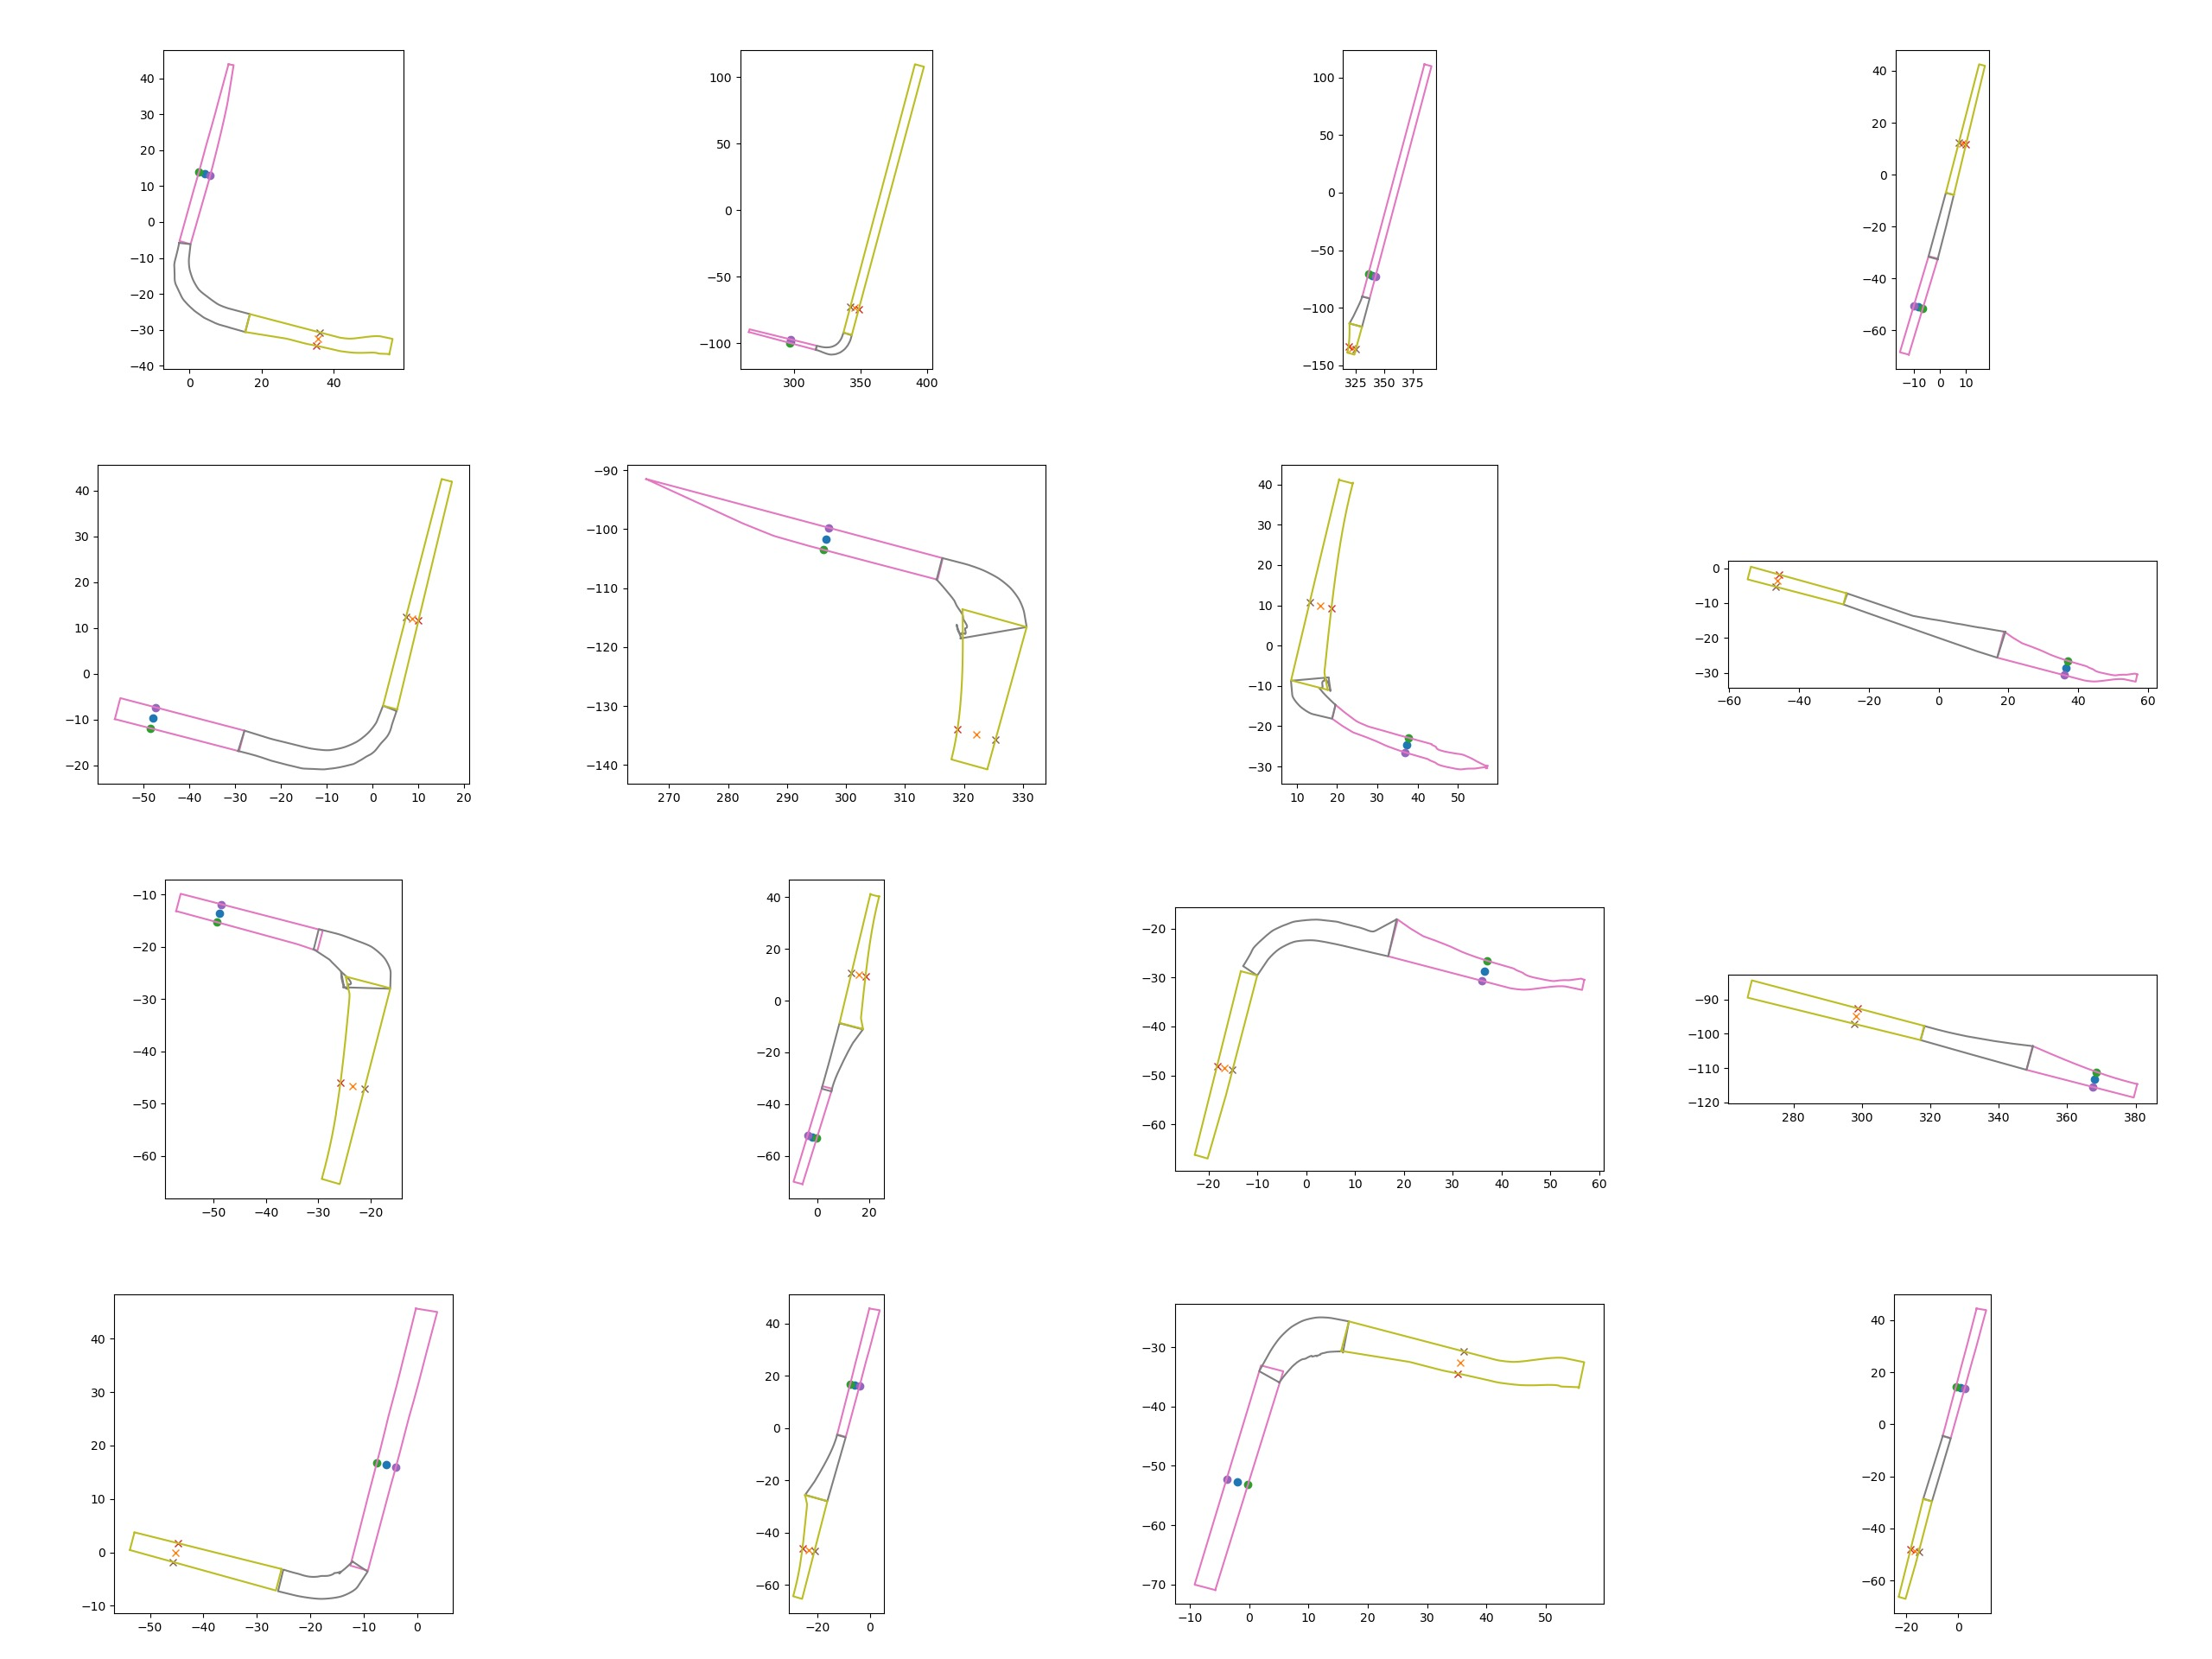
\includegraphics[width=0.5\textwidth]{images/feature_borregasave_maps}
%     \caption{Borregas Ave trajectories based 10-by-10 cells map.}
% \end{figure}

% \begin{figure}[H]
%   \centering
%     \includegraphics[width=0.5\textwidth]{images/two_roads_same_cell.png}
%     \caption{Example of two roads that belong to the same cell.}
% \end{figure}

% \begin{figure}[H]
%   \centering
%     \includegraphics[width=0.5\textwidth]{images/roads_different_cell.png}
%     \caption{Example of three roads taken from different (distant) cells.}
% \end{figure}


\subsection{Generating Test Cases}
\tool generates a set of diversified driving scenarios as a combination of lanelets. So it needs to transform them into test cases that can be executed as simulations and result either in passing or failing.
\tool does so by implementing introductory test oracles that check if the ego-vehicle reaches the target location after the intersection within a predefined timeout and by using simple geometric transformations to place the ego-vehicle in the starting position and rotate it according to the geometry of the initial lanelets.

However, doing so is not enough since the simulations may include additional elements, such as traffic lights that affect the test result. For example, if the ego-vehicle needs to pass a controlled intersection and the traffic light is red, the ego-vehicle must stop in front of it, which may cause the timeout to trigger a false positive. Therefore, to avoid such false positives, \tool programs any traffic lights on the expected trajectories to turn green when the ego-vehicle approaches them.

\subsection{Spicing Up the Test Cases}
The tests generated by \tool are plain: they stress the ability of the ego-vehicle to plan trajectories that pass intersections and keep the lane but involve no other element besides the ego-vehicle and possibly traffic lights. 
Therefore, we illustrate how those test cases can be extended by placing static obstacles on the course of the ego-vehicle by letting  \tool place parked vehicles on the roads. 

Our approach to ``spice up'' the test cases starts from an existing driving scenario and generate tests by placing NPC vehicles predefined positions between the ego-vehicle's initial position (i.e., the starting point of the driving scenario) and the intersection. Placing NPC vehicles results is partially or entirely occlusions of the lane, forcing the ego-vehicle to swerve or change lane. Default occlusions are partial, and \tool causes them by placing an NPC vehicle on the left or right side of the lane. Additionally, if the geometry of the intersection allows it, \tool places an NPC in the middle of the lane in front of the ego-vehicle, forcing it to switch lanes before entering the intersection.

In summary, on top of the test cases that \tool can generate from a given map, testers can quickly generate up to four times more test cases by simply adding NPC vehicles in front of the ego-vehicle. As we did before, we decided to place up to one NPC vehicle per test case to keep the test cases as simple and understandable as possible.

\subsection{Prototype}
\tool is implemented as a Python (version 3.9) command-line application and currently integrated with the SVL driving simulator.\footnote{\href{https://www.svlsimulator.com/}{https://www.svlsimulator.com/}} 
% Specifically, we use Python 3.9, the libraries listed in the requirements.txt file, and the maps in OpenDrive format available in the SVL simulator.
%
We tested \tool on Ubuntu 20.04.2 LTS running the SVL Simulator version 2021.01 and Apollo Baidu version 6.0 \footnote{\href{https://apollo.auto/}{https://apollo.auto/}} in accordance to the rules of the \challenge.

\section{Achieved Results and Found Problems}
To evaluate \tool, we applied it to test Apollo Baidu on the following five maps that were available on the SVL Web site at the time the \challenge took place:

\begin{enumerate}
 \item Cube Town
 \item Borregas Avenue
 \item Shalun
 \item GoMentum
 \item San Francisco
\end{enumerate}

We selected those five maps according to the following criteria: size, number of intersections, and compatibility with the opendrive2lanelets library (see column \emph{Intersections} in Table~\ref{tab:results} and figures~5--9).

As reported in Table~\ref{tab:results}, using those five maps, \tool identified more than a hundred intersections and generated more than a thousand driving scenarios that do not involve NPV vehicles. From those scenarios, \tool selected up to 50\% test cases for the execution using features maps, whereas using distance, it selected considerably more cases.

\begin{table}[t]
    \centering
      \caption{\tool's Evaluation Results}
      \label{tab:results}
      \begin{tabular}{lrrrr}
        \toprule
        \multicolumn{1}{c}{\textbf{Map Name}}&
        \multicolumn{1}{c}{\textbf{Intersections}}&
        \multicolumn{1}{c}{\textbf{Total Tests}}&
        \multicolumn{2}{c}{\textbf{Selected Tests}} \\
        & & & Similarity & Feature Map\\
        \midrule
        Cube Town & 2 & 12 & 8 & 5\\
        Borregas Ave & 2 & 28 & 20 & 16\\
        Shalun & 14 & 149 & 124 & 33\\
        Gomentum & 25 & 126 & 110 & 25\\
        San Francisco & 89 & 806 & 535 & 52\\
        \bottomrule
      \end{tabular}
\end{table}



\begin{figure*}[!tp]
\minipage{0.31\textwidth}
  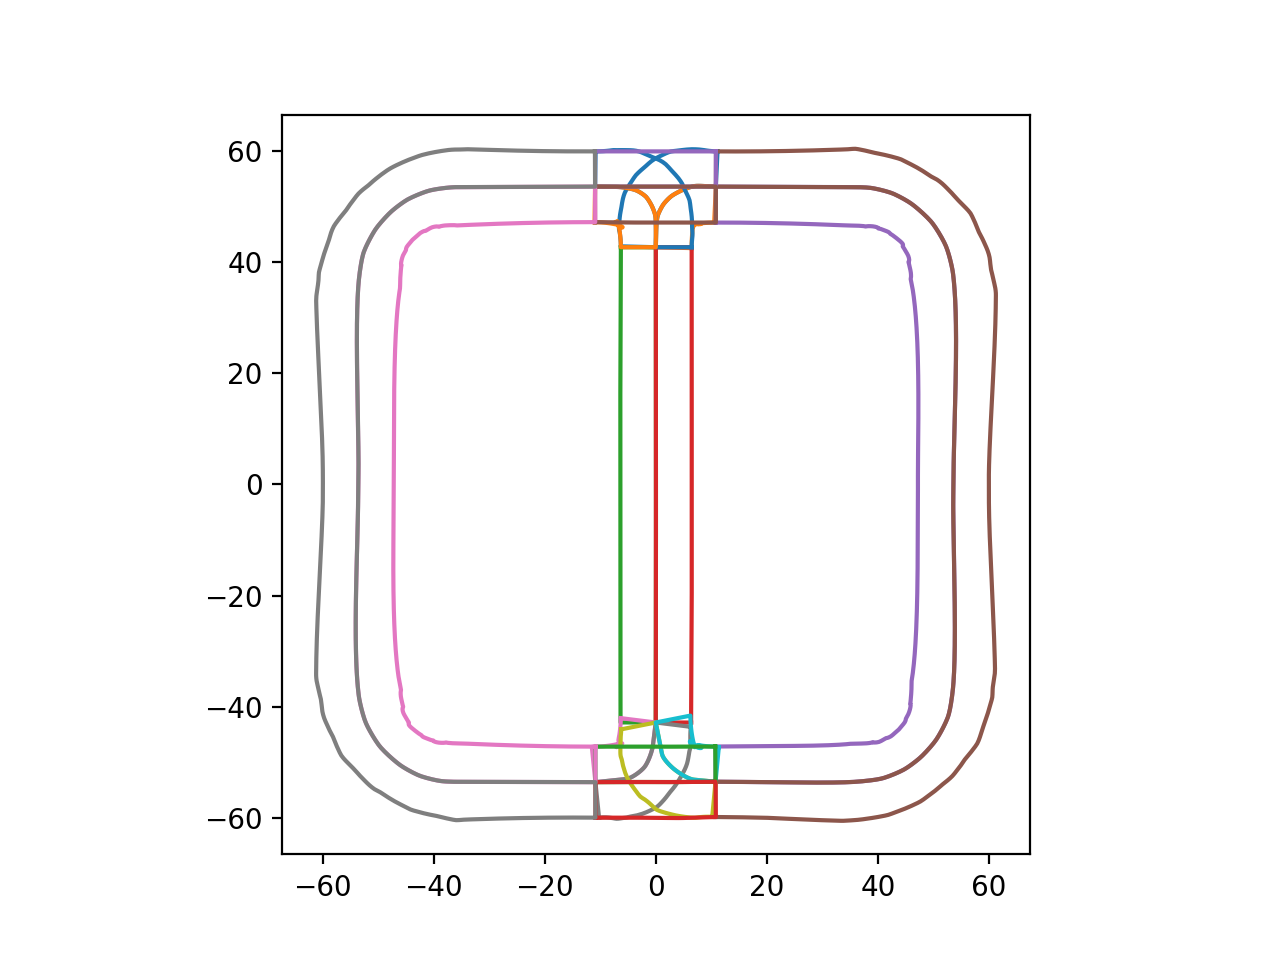
\includegraphics[width=\linewidth]{images/map_cubetown}
  \includegraphics[width=\linewidth]{images/feature_cubetown}
  \caption{Cube Town map.}
\endminipage\hfill
\minipage{0.31\textwidth}
  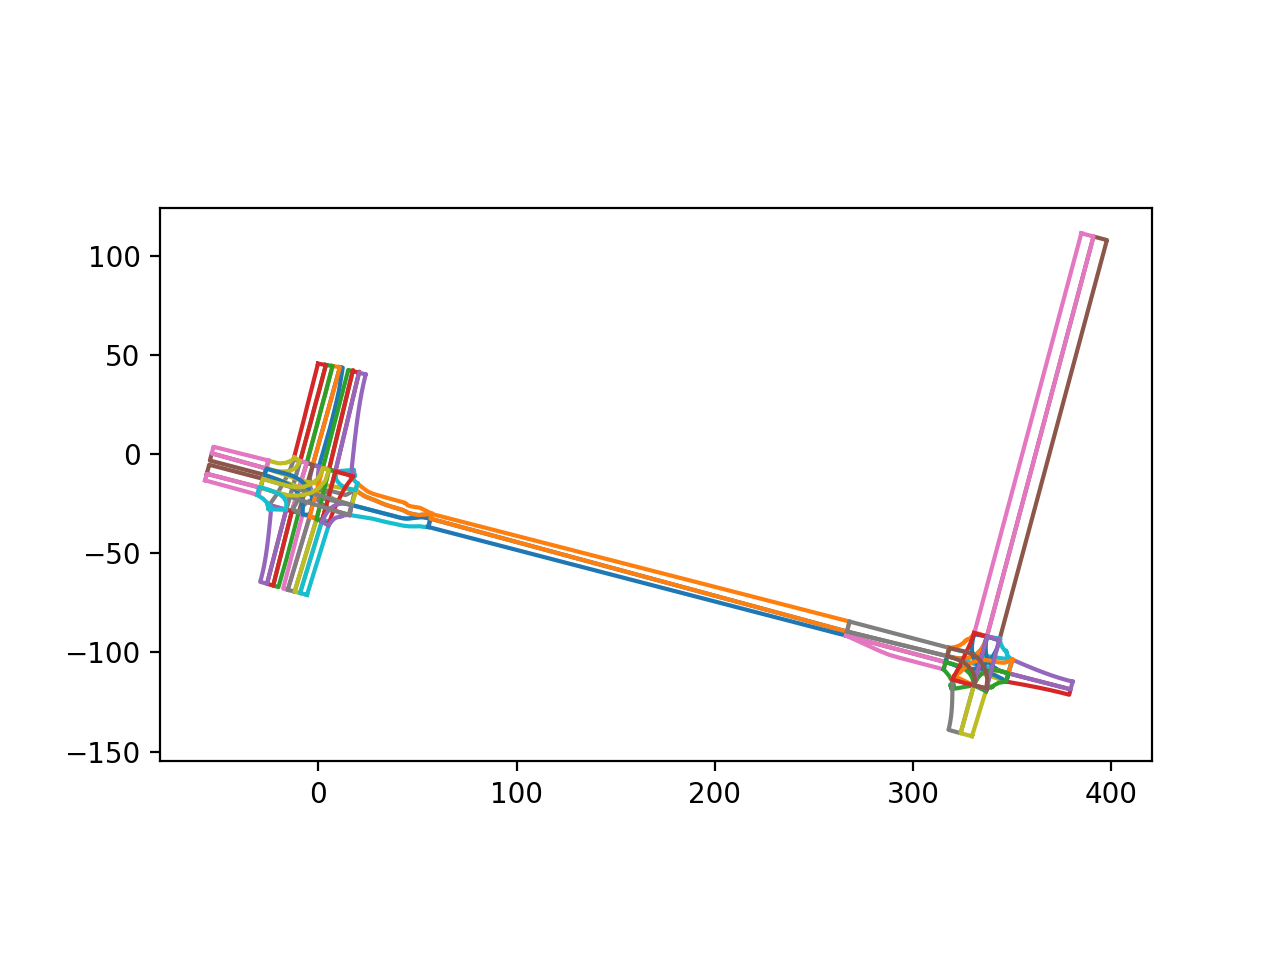
\includegraphics[width=\linewidth]{images/map_borregasave}
  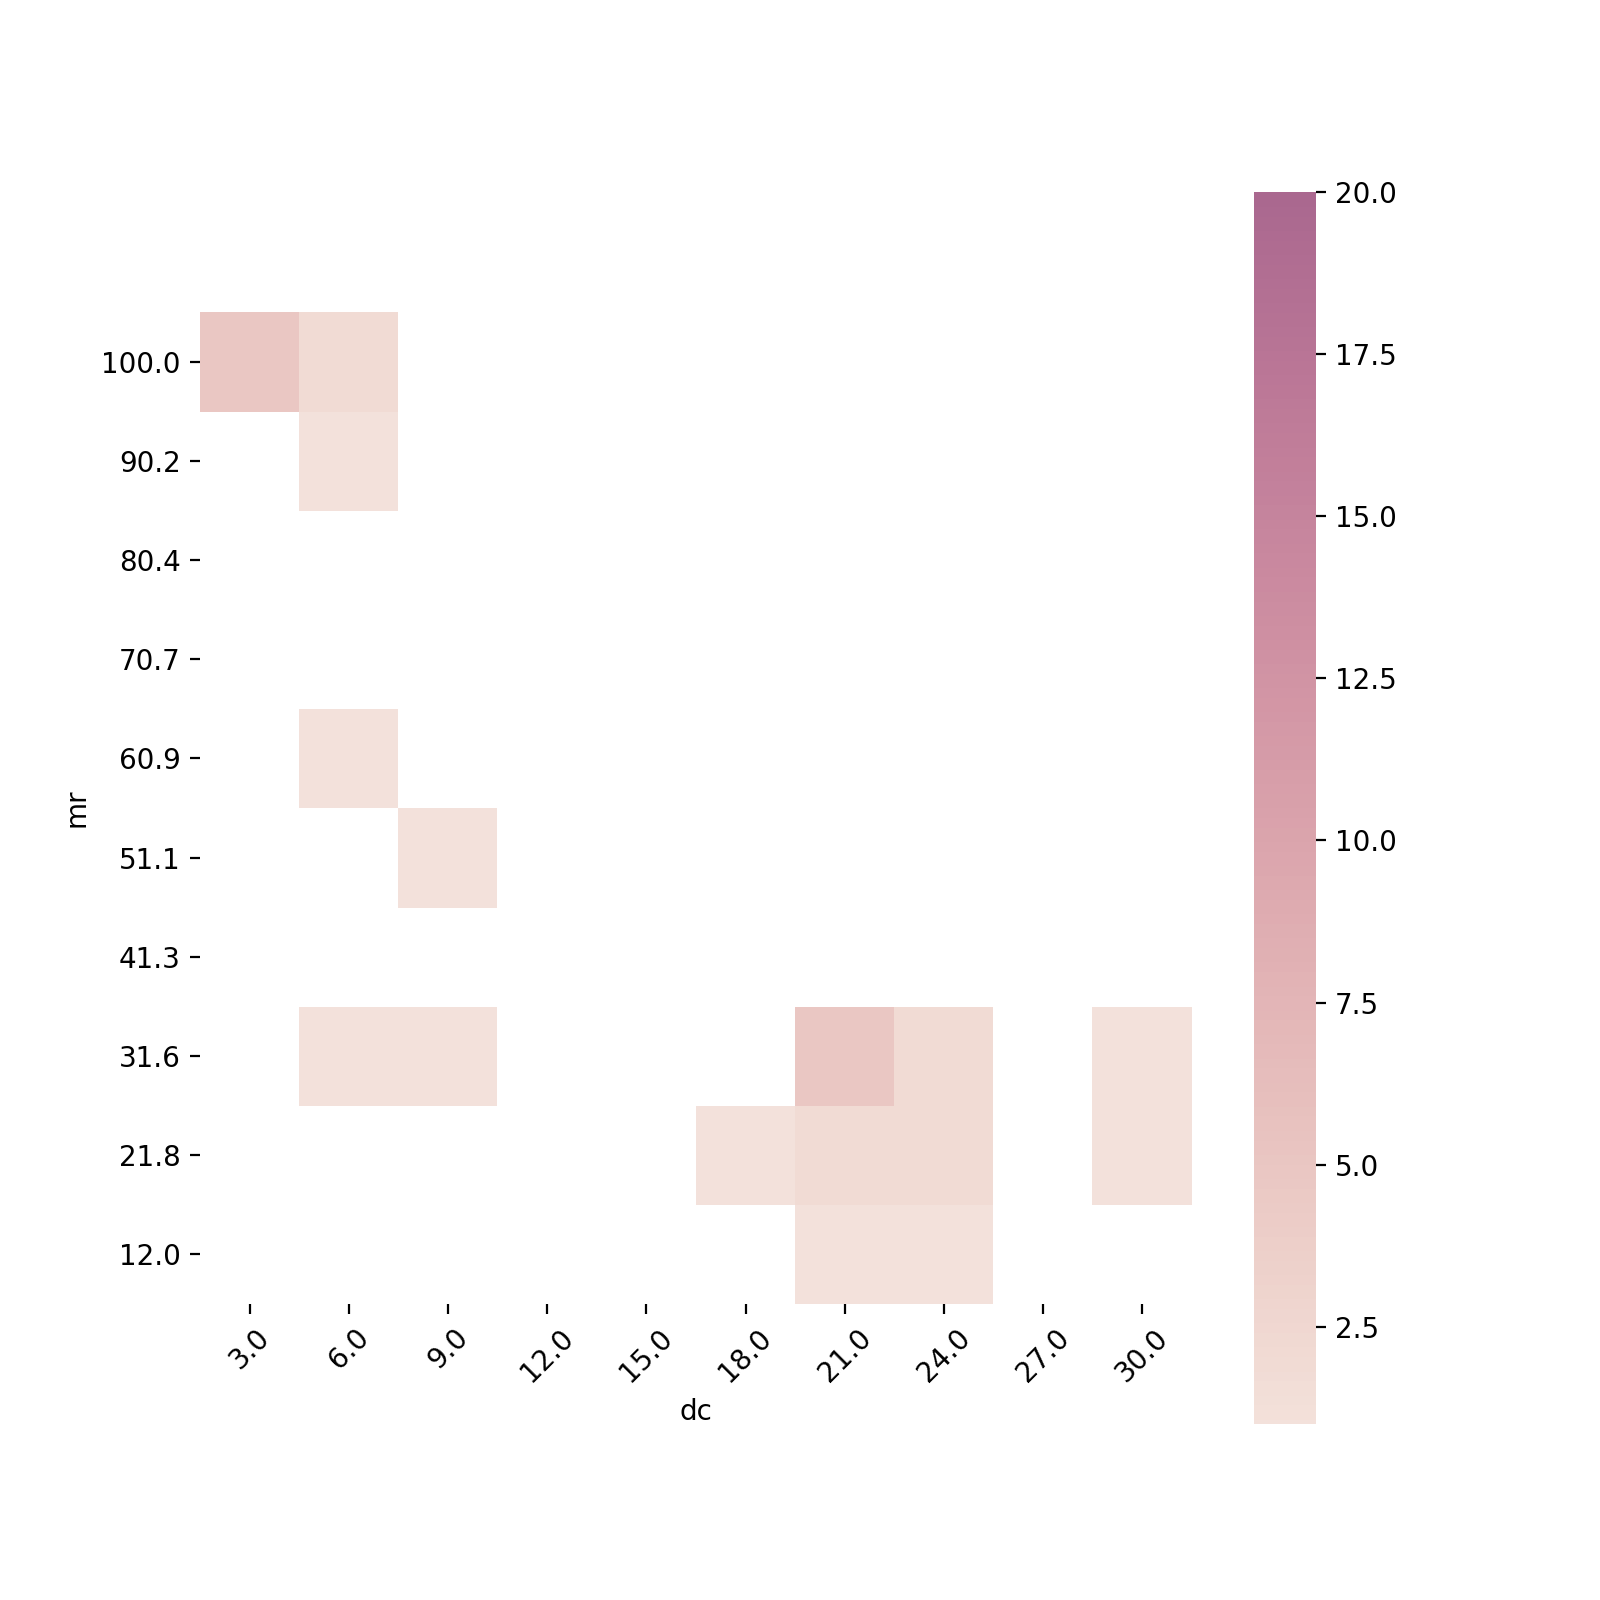
\includegraphics[width=\linewidth]{images/feature_borregasave}
  \caption{Borregas Ave map.}
\endminipage\hfill
\minipage{0.31\textwidth}%
  \includegraphics[width=\linewidth]{images/map_shalun}
  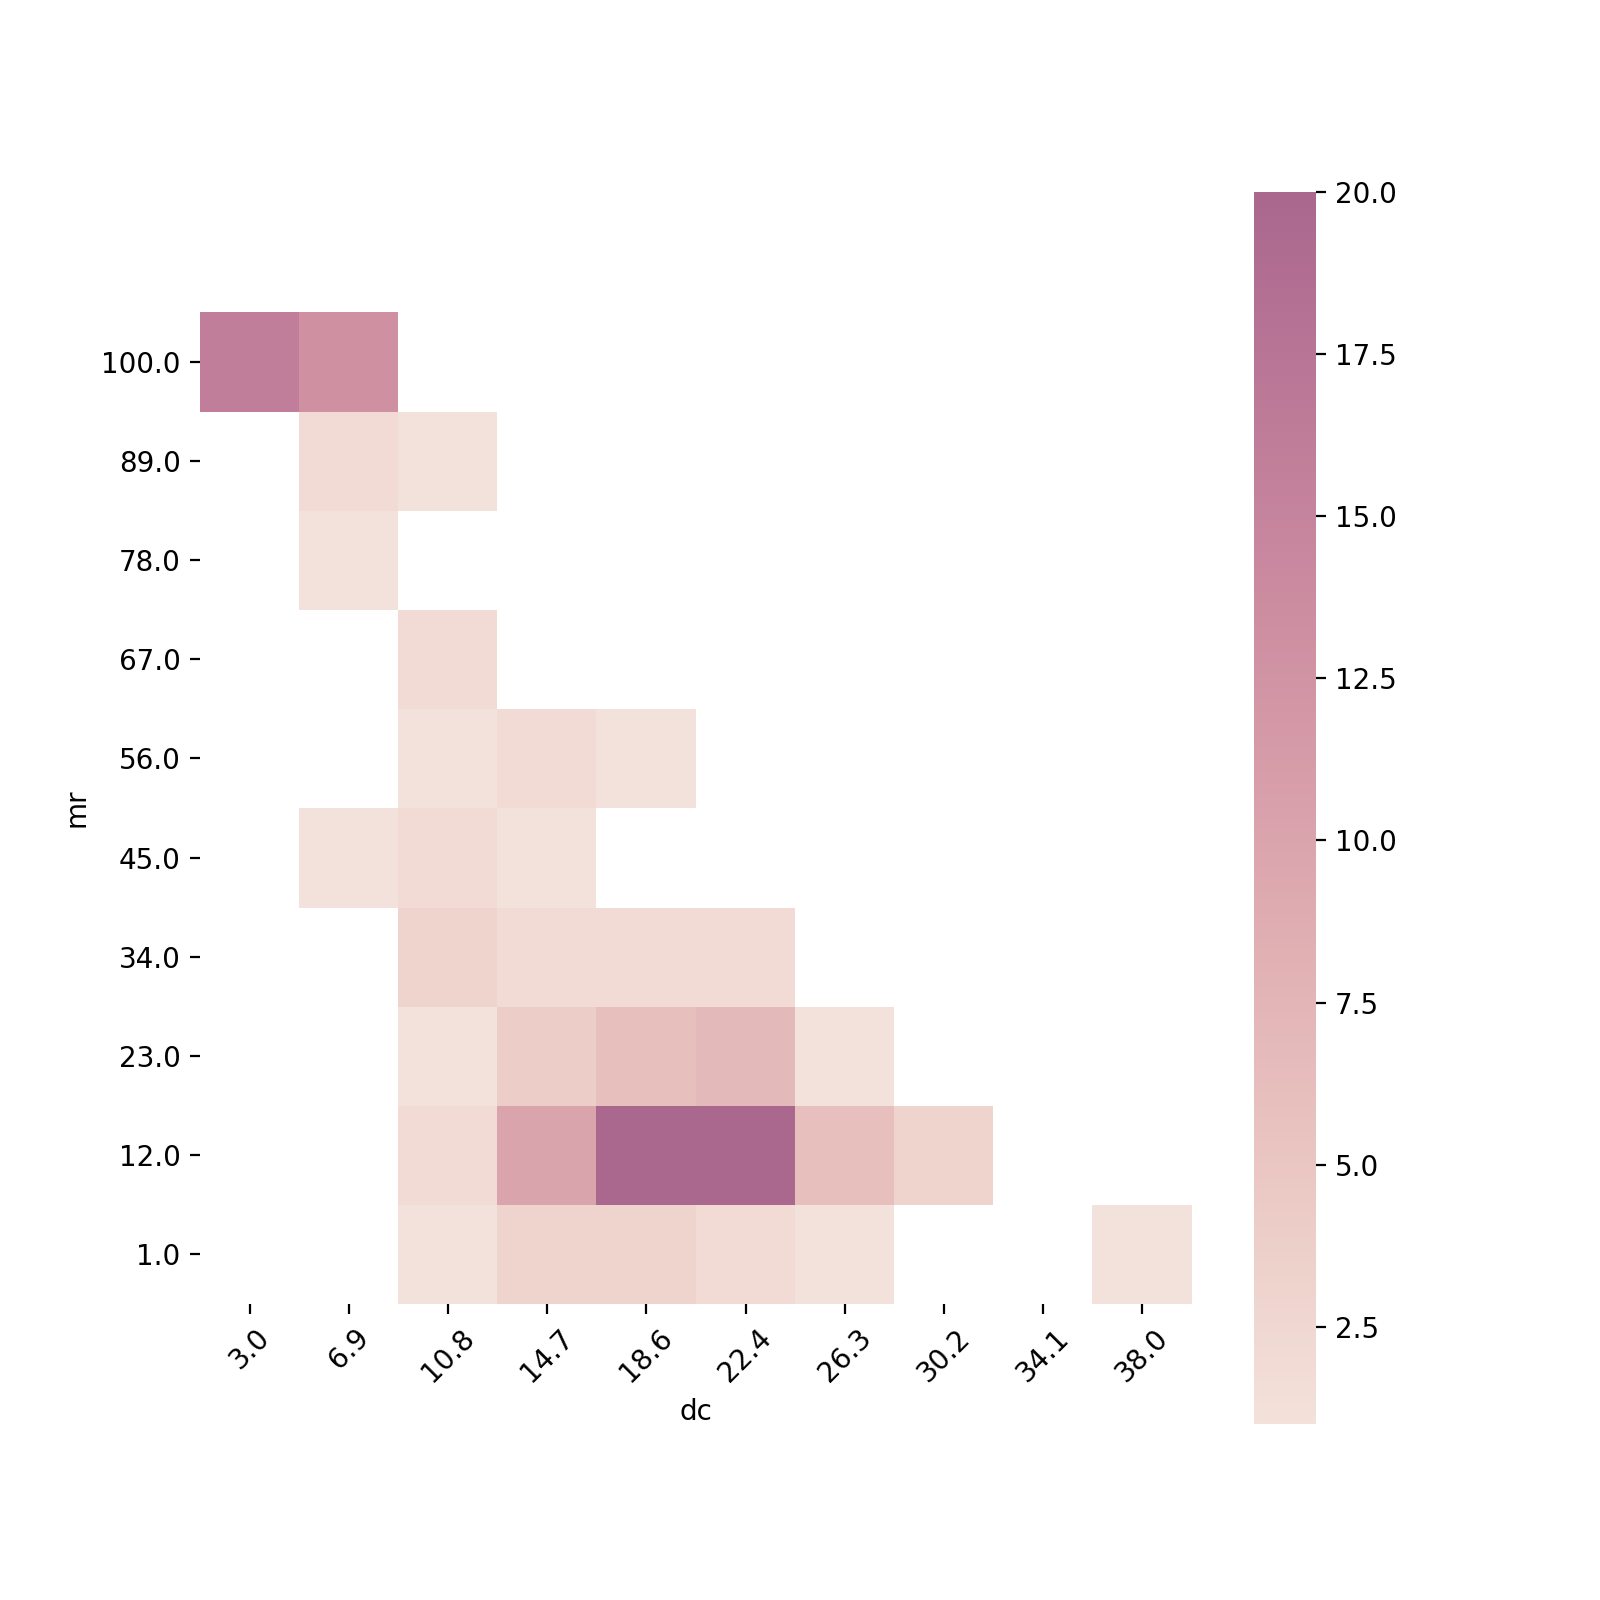
\includegraphics[width=\linewidth]{images/feature_shalun}
  \caption{Shalun map.}
\endminipage

\minipage{0.31\textwidth}%
  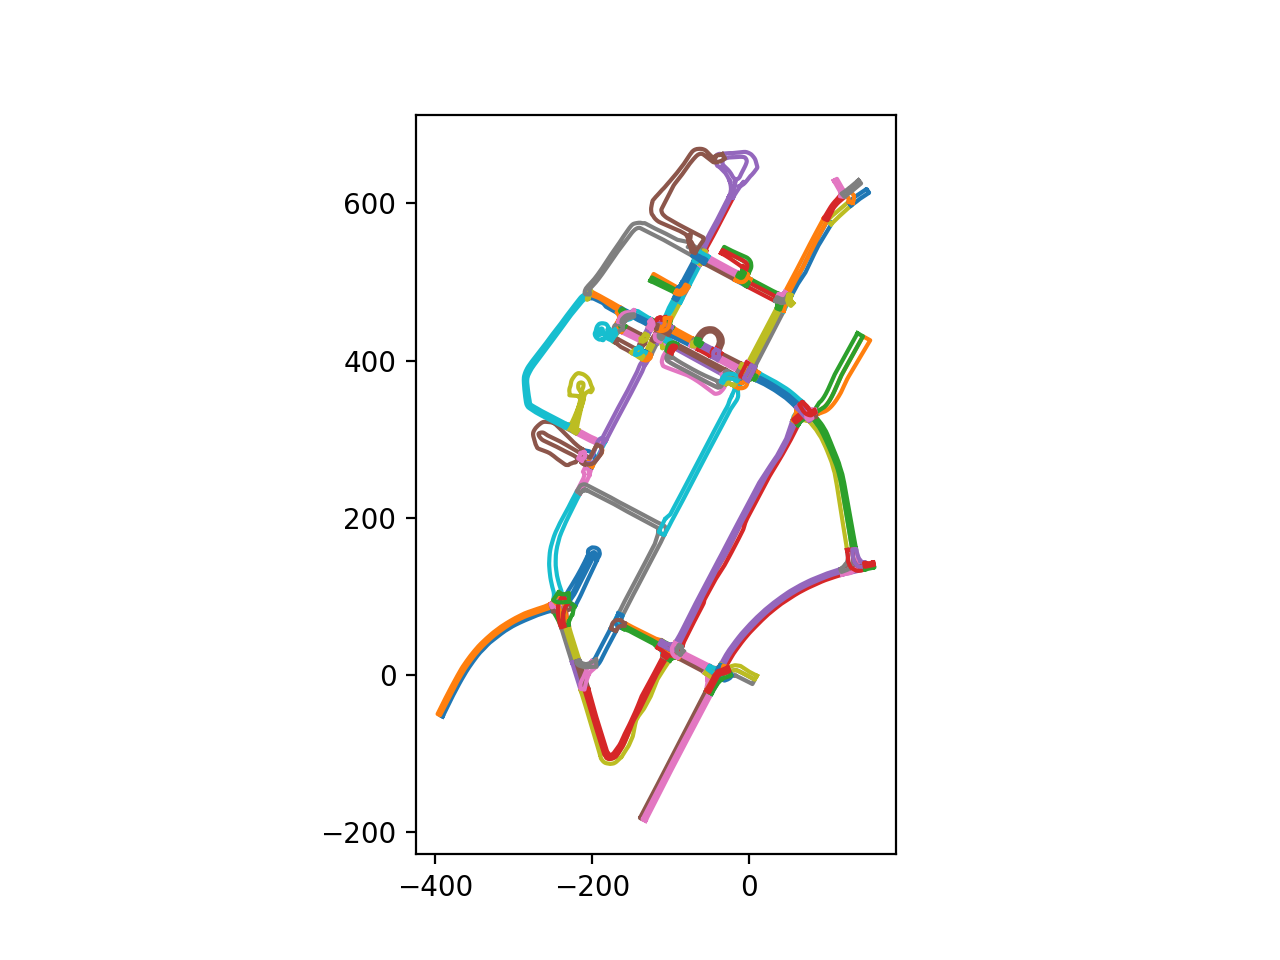
\includegraphics[width=\linewidth]{images/map_gomentum}
  \includegraphics[width=\linewidth]{images/feature_gomentum}
  \caption{Gomentum map.}
\endminipage\hfill
\minipage{0.31\textwidth}%
  \includegraphics[width=\linewidth]{images/map_sanfrancisco.png}
  \includegraphics[width=\linewidth]{images/feature_sanfrancisco.png}
  \caption{San Francisco map.}
\endminipage
\minipage{0.31\textwidth}%
    \includegraphics[width=\linewidth]{images/map_sanfrancisco.png}
\endminipage
\label{fig:feature-maps-results}
\end{figure*}

The execution of the generated test cases resulted in failed test cases caused by the test subject not reaching the target location in time. Since we take extra care to remove all possible causes of false positives (e.g., traffic lights and random traffic), this result suggests that the test subject could not plan a suitable trajectory in some cases.

\section{Future Work}

In the hope of capturing the intended aim of the challenge, we brainstormed possible ideas to implement for future work. We tried to "think out-of-the-box" while remaining pragmatic. Below we summarize two of such ideas.

\paragraph{Parking Lot Madness}
Create scenarios that take place inside parking lots to test features like Tesla's "Smart Summon". The idea is to check if the ego-vehicle can safely drive from a parking spot to the parking lot's exit despite pedestrians and other vehicles. Our vision is to generate scenarios by placing the ego-vehicle in different parking spots and controlling the placement and movement of non-ego cars and pedestrians to create various situations.

\paragraph{To Pass or Not to Pass?}
Check the behaviour of the ego vehicle while handling controlled intersections. The idea is to take any map, find where controlled intersections and traffic lights are, and (automatically) generate scenarios where the car must pass the various controlled intersections.
%
Concrete tests can be generated by changing which controlled intersection to pass, the direction that ego-vehicle should follow (e.g., turn right, go straight), and directly acting upon the traffic lights (e.g., flashing lights, turn it off).
%
Alternatively, we can also place the ego car in the middle of those intersections and try to "trap it there" by controlling the traffic lights. This additional arrangement will let us check whether the vehicle can adequately free controlled intersections or get stuck in the middle of it.

% References
\bibliographystyle{IEEEtran}
\bibliography{biblio}

\end{document}
